\documentclass{article}
\usepackage{tikz}
\usepackage{amsmath}
\usepackage{amssymb}
\usepackage{graphicx}
\usepackage{xcolor}
\usepackage{colortbl}
\usepackage[margin=1in]{geometry}

% Add TikZ libraries
\usetikzlibrary{positioning}
\usetikzlibrary{arrows.meta}
\usetikzlibrary{calc}

\title{Scoreformer: Interactive Matrix Flow Analysis}
\author{Detailed Architecture Analysis}
\date{\today}

\begin{document}
\maketitle

\section{Input Layer Visualization}

\begin{figure}[ht]
\centering
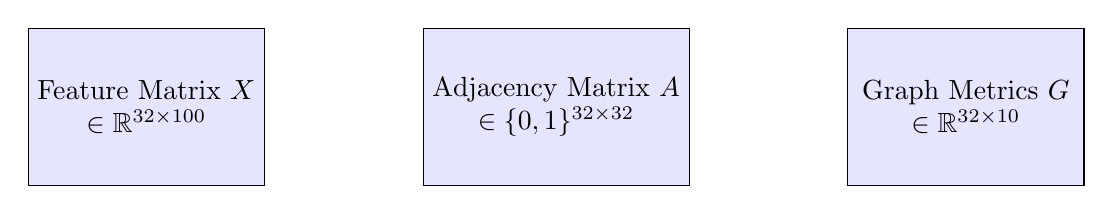
\begin{tikzpicture}[
    box/.style={draw, minimum width=3cm, minimum height=2cm, align=center, fill=blue!10},
    arrow/.style={->, thick}
]
    % Input matrices with dimensions
    \node[box] (X) {Feature Matrix $X$\\$\in \mathbb{R}^{32 \times 100}$};
    
    \node[box, right=2cm of X] (A) {Adjacency Matrix $A$\\$\in \{0,1\}^{32 \times 32}$};
    
    \node[box, right=2cm of A] (G) {Graph Metrics $G$\\$\in \mathbb{R}^{32 \times 10}$};
\end{tikzpicture}
\caption{Input Matrices with Sample Values}
\end{figure}

\section{Attention Mechanism}

\begin{figure}[ht]
\centering
\begin{tikzpicture}[
    box/.style={draw, minimum width=2.8cm, minimum height=1.8cm, align=center},
    att/.style={draw, minimum width=2.5cm, minimum height=1.5cm, fill=red!10}
]
    % Query, Key, Value matrices
    \node[box] (Q) {Query $Q$\\$WX$};
    \node[box, right=2cm of Q] (K) {Key $K$\\$WX$};
    \node[box, right=2cm of K] (V) {Value $V$\\$X$};
    
    % Attention score computation
    \node[att, below=2cm of K] (att) {Attention Scores\\$\text{softmax}(\frac{QK^T}{\sqrt{d_k}})$};
    
    % Output
    \node[box, below=2cm of att] (out) {Output\\$\text{Attention}(Q,K,V)$};
    
    % Arrows
    \draw[arrow] (Q) -- (att);
    \draw[arrow] (K) -- (att);
    \draw[arrow] (V) -- (att);
    \draw[arrow] (att) -- (out);
\end{tikzpicture}
\caption{Self-Attention Mechanism}
\end{figure}

\section{DNG Score Formation}

\begin{figure}[h]
\centering
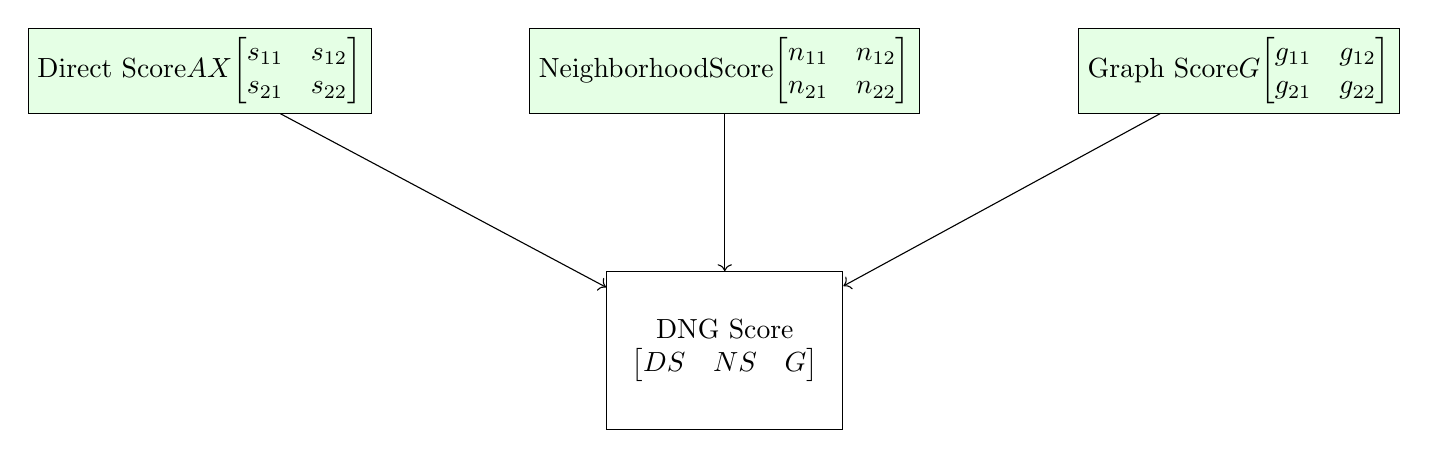
\begin{tikzpicture}[
    box/.style={draw, minimum width=3cm, minimum height=2cm, align=center},
    score/.style={draw, fill=green!10}
]
    % Direct Score
    \node[score] (DS) {Direct Score\\$AX$\\
    $\begin{bmatrix}
    s_{11} & s_{12}\\
    s_{21} & s_{22}
    \end{bmatrix}$};
    
    % Neighborhood Score
    \node[score, right=2cm of DS] (NS) {Neighborhood\\Score\\
    $\begin{bmatrix}
    n_{11} & n_{12}\\
    n_{21} & n_{22}
    \end{bmatrix}$};
    
    % Graph Score
    \node[score, right=2cm of NS] (GS) {Graph Score\\$G$\\
    $\begin{bmatrix}
    g_{11} & g_{12}\\
    g_{21} & g_{22}
    \end{bmatrix}$};
    
    % Combined Score
    \node[box, below=2cm of NS] (DNG) {DNG Score\\
    $\begin{bmatrix}
    DS & NS & G
    \end{bmatrix}$};
    
    % Arrows with concatenation
    \draw[->] (DS) -- (DNG);
    \draw[->] (NS) -- (DNG);
    \draw[->] (GS) -- (DNG);
\end{tikzpicture}
\caption{DNG Score Formation Process}
\end{figure}

\section{Final Output Layer}

\begin{figure}[h]
\centering
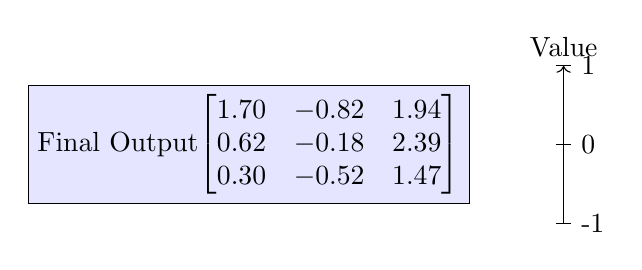
\begin{tikzpicture}[
    box/.style={draw, minimum width=3cm, minimum height=2cm, align=center},
    heat/.style={draw, fill=blue!10}
]
    % Final output heatmap
    \node[heat] (out) {Final Output\\
    $\begin{bmatrix}
    1.70 & -0.82 & 1.94\\
    0.62 & -0.18 & 2.39\\
    0.30 & -0.52 & 1.47
    \end{bmatrix}$};
    
    % Add colorbar
    \begin{scope}[shift={(4,0)}]
        \draw[->] (0,-1) -- (0,1) node[above] {Value};
        \foreach \y/\v in {-1/-1, 0/0, 1/1} {
            \draw (-0.1,\y) -- (0.1,\y) node[right] {\v};
        }
    \end{scope}
\end{tikzpicture}
\caption{Final Output Matrix with Values}
\end{figure}

\section{Complete Architecture Flow}

\begin{figure}[ht]
\centering
\begin{tikzpicture}[
    box/.style={draw, minimum width=3cm, minimum height=2cm, align=center},
    proc/.style={draw, minimum width=2cm, minimum height=1.5cm, align=center},
    >=Stealth,  % Arrow style
    node distance=2cm
]
    % Input layer
    \node[proc] (input) {Input Matrix};
    
    % Processing nodes
    \node[proc, below left=of input] (direct) {Direct Score};
    \node[proc, below=of input] (jaccard) {Jaccard Similarity};
    \node[proc, below right=of input] (graph) {Graph Metrics};
    
    % DNG formation
    \node[box, below=2cm of jaccard] (dng) {DNG Scores};
    
    % Transformer
    \node[proc, right=2cm of dng] (trans) {Transformer};
    
    % Final output
    \node[box, right=2cm of trans] (output) {Output};
    
    % Connections with proper arrow style
    \draw[->] (input) -- (direct);
    \draw[->] (input) -- (jaccard);
    \draw[->] (input) -- (graph);
    \draw[->] (direct) -- (dng);
    \draw[->] (jaccard) -- (dng);
    \draw[->] (graph) -- (dng);
    \draw[->] (dng) -- (trans);
    \draw[->] (trans) -- (output);
\end{tikzpicture}
\caption{Complete Scoreformer Architecture}
\end{figure}

\end{document}